\section{Klassendiagram}
\subsection{Overzicht}

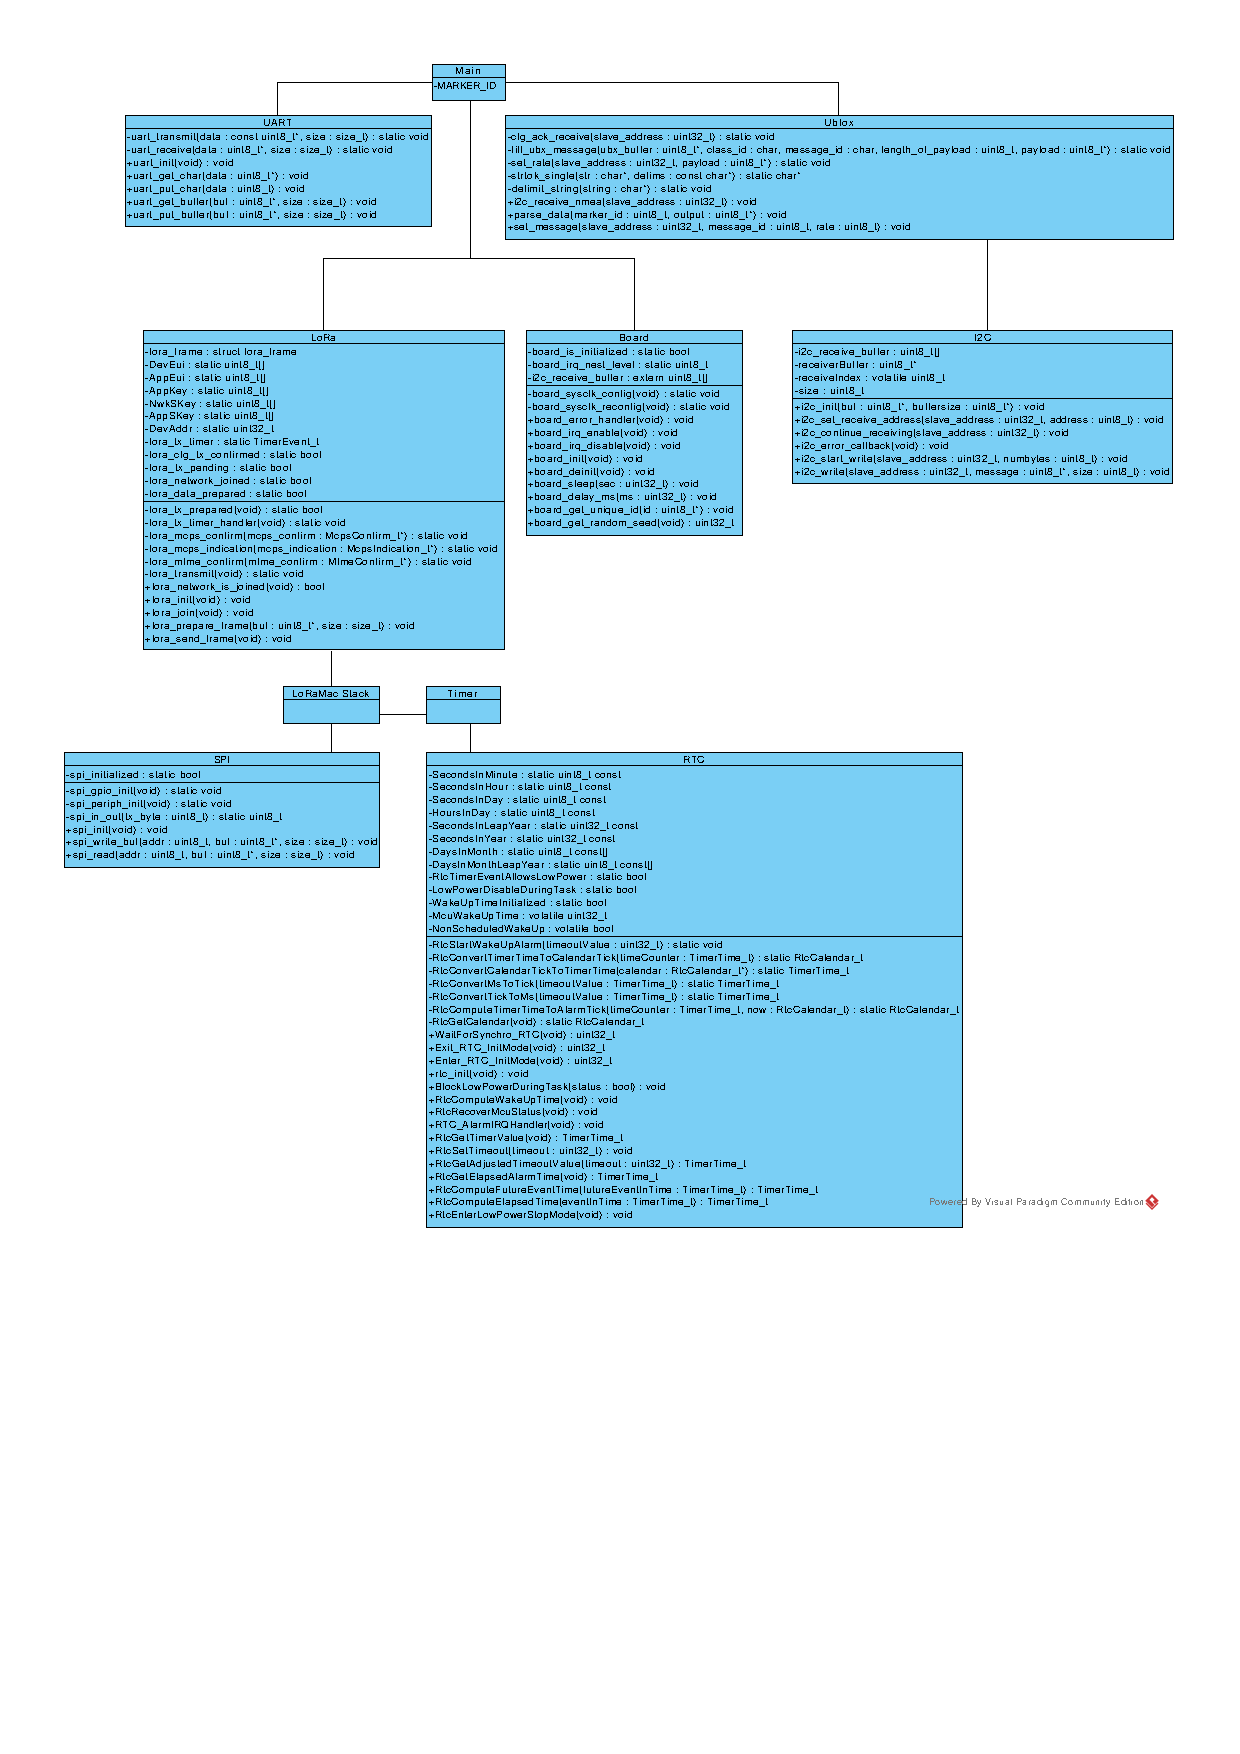
\includegraphics[width=0.9\linewidth]{technical/class_diagram.pdf}

\subsection{Klassen}
\subsubsection{Node}
\paragraph{Attributen}
De Node klasse heeft een uniek ID. Met een boolean type kan worden aangegeven of de Node een referentiestation is. De gps\_data bevat de locatiegegevens, en de payload bevat de gefilterde gps\_data.

\paragraph{Functies}
\begin{itemize}
    \item \texttt{init\_hardware()} initialiseert de hardware/peripherals.
    \item \texttt{init\_lora()} initialiseert de LoRaWAN netwerk stack.
    \item \texttt{init\_gps()} initialiseert de GPS module.
    \item \texttt{gps\_acquire()} zoekt naar satellieten.
    \item \texttt{gps\_measure(struct gps\_data)} schrijft een GPS-meting weg in een gps\_data struct.
    \item \texttt{lora\_register(id, ref\_station)} registreert de Node in het netwerk.
    \item \texttt{lora\_data\_prepare(struct gps\_data)} verpakt gps\_data in een payload struct, om via het LoRa netwerk verstuurd te worden.
    \item \texttt{lora\_data\_send(struct payload)} verstuurt de payload.
    \item \texttt{sleep(sec)} zet het device in slaapmodus voor
\end{itemize}

\subsubsection{Referentiestation}
Het referentiestation is een Node waarvan de \texttt{ref\_station} \texttt{true} is. De positie van dit referentiestation is met hoge nauwkeurigheid vastgelegd, om middels DGPS een correctie uit te kunnen voeren.

Het referentiestation stuurt DGPS-data.

\subsubsection{Gateway}
De gateway ontvangt data van alle Nodes en stuurt de data door naar een applicatieserver, waar het vervolgens in een database wordt weggeschreven.

\subsubsection{Database}
De database bevat de GPS-gegevens waar een correctie op is uitgevoerd. Deze data wordt gebruikt voor de weergave in een Google API.

\subsubsection{GPS-data}
Het GPS-data struct bevat een (talker) ID van de GPS-module, tijd in UTC-format, en de locatiegegevens in latitude, longitude en altitude.

\subsubsection{DGPS-data}
Het DGPS-data struct ziet er hetzelfde uit als GPS-data, met een aanvulling van foutcorrectie attributen.